\documentclass[twocolumn]{rbef}
\usepackage{lipsum}

\usepackage{bbm}
\usepackage{subfig}

\newcommand{\1}{\mathbbm{1}}
\newcommand{\s}{\mathcal{S}}
\newcommand{\T}{\mathcal{T}}
\newcommand{\A}{\mathcal{A}}
\newcommand{\ket}{\rangle}
\newcommand{\bra}{\langle}

\newtheorem{defi}{Definição}
\newtheorem{theorem}{Teorema}
\newtheorem{acknowledgement}[theorem]{Acknowledgement}
\newtheorem{algorithm}[theorem]{Algorithm}
\newtheorem{axiom}[theorem]{Axiom}
\newtheorem{claim}[theorem]{Claim}
\newtheorem{conclusion}[theorem]{Conclusion}
\newtheorem{condition}[theorem]{Condition}
\newtheorem{conjecture}[theorem]{Conjecture}
\newtheorem{corollary}[theorem]{Corollary}
\newtheorem{criterion}[theorem]{Criterion}
\newtheorem{definition}[theorem]{Definition}
\newtheorem{example}[theorem]{Example}
\newtheorem{exercise}[theorem]{Exercise}
\newtheorem{lemma}[theorem]{Lemma}
\newtheorem{notation}[theorem]{Notation}
\newtheorem{problem}[theorem]{Problem}
\newtheorem{proposition}[theorem]{Proposition}
\newtheorem{remark}[theorem]{Remark}
\newtheorem{solution}[theorem]{Solution}
\newtheorem{summary}[theorem]{Summary}
\newenvironment{proof}[1][Proof]{\noindent\textbf{#1.} }{\ \rule{0.5em}{0.5em}}

\titulocabecalho{Sobre Dinâmica de Partículas Carregadas em Campos Elétrico e Magnético Estáticos}
\autorcabecalho{M. L. Medeiros and A. C. Santos}

\numeracao{01}
\volume{01}
\numero{01}
\ano{2019}
\doi{http://dsbd.leg.ufpr.br/tcc}
% \tipodeartigo{TCC DSBD}
\tipodeartigo{Especialização em Data Science \& Big Data}
% \addtocounter{page}{566} %% \setcounter produces extra white page!!! use ===\addtocounter===

\author[1]{Marciano L. Medeiros}

\affil[1]{Departamento de Física, Universidade Regional do Cariri
  Av. Leão Sampaio 107, Triângulo, 63041-082, Juazeiro do Norte, CE,
  Brasil\thanks{\href{emailto:martefeynman@gmail.com}{martefeynman@gmail.com}}
}

\author[2]{Alan C. Santos}

\affil[2]{Instituto de Física, Universidade Federal Fluminense
  Av. General Milton Tavares de Sousa s/n, Gragoatá, 24410-346, Niterói,
  RJ, Brasil\thanks{\href{emailto:alancs@if.uff.br}{alancs@if.uff.br}}
}

\titulo{Sobre Dinâmica de Partículas Carregadas em Campos Elétrico e
  Magnético Estáticos}

\subtitulo{On Dynamic of charged particles in Electric and Magnetic
  statics fields}

% -----------------------------------------------------------------------

\begin{document}

\begin{primeirapagina}

  % \begin{center}
  %   \vspace{-12pt} \small{Recebido em xxx. Aceito em xxx}
  % \end{center}

  \begin{abstract}
    Um desenvolvimento didático para determinar a solução da
    equação de movimento para uma partícula carregada imersa em
    uma região na presença de campos elétrico e magnéticos
    estáticos genéricos é proposto. Nossa proposta tem como
    alicerce a vantagem de, utilizando as propriedades da
    transformada de Laplace, podermos mapear um sistema de
    equações diferenciais não-homogêneas de segunda ordem no
    problema simples de encontrar as soluções de um sistema linear
    de equações. A partir da solução mais geral possível para o
    sistema, estudamos alguns casos particulares e recuperamos de
    forma simples alguns resultados já existentes na literatura. A
    fim de motivar nosso estudo, partimos do Teorema de Ehrenfest
    e discutimos como os resultados obtidos para o caso clássico
    podem ser interpretados na sua versão quântica.
    \palavraschave{movimento de cargas, campos elétrico e
      magnético, trajetória, análogo quântico}

  \end{abstract}

  \begin{otherlanguage}{english}


    \begin{abstract}
      A didactic development to determinate the solution of the
      motion equations for a charged particle under influence of
      electric and magnetic static fields is proposed. Our proposed
      uses the advantages and proprieties of the Laplace’s
      transformation, to map a system of N non-homogeneous
      differential equations of second order in a system composed by
      N linear equations. From the solution more general for
      dynamics of the system, we study some particular cases to
      recover, of a simple way, the results present in the
      literature. In order to give a motivation to our study, we use
      the Ehrenfest’s theorem and we discuss as the classical
      results can be interpreted in its quantum version.
      \keywords{Charge moving, electric and magnetic fields,
        trajectory, quantum analogue}

    \end{abstract}
  \end{otherlanguage}

\end{primeirapagina}
\saythanks

\section{Introdução}

De forma elegante a Mecânica Newtoniana (Mecânica Clássica)
permite-nos entender o comportamento de partículas que estão
sujeitas a determinadas forças e condições iniciais
\cite{Sommerfeld,Landau}. Porém o tamanho de sistemas físicos
impõe um limite sobre o regime de validade da Mecânica Clássica,
de modo que sistemas do tamanho do átomo de Hidrogênio, por
exemplo, podem apresentar comportamentos peculiares à luz da
Mecânica Clássica. Porém há casos onde o tratamento clássico do
comportamento de um sistema pode nos dá informações relevantes
sobre o sistema de interesse. Um exemplo é o de uma partícula de
carga $q$ na presença de campos magnético $\vec{B}$ e elétrico
$\vec{E}$ estáticos, como discutiremos aqui.

É conhecido que quando uma partícula penetra em uma região do
espaço onde há campos magnético e elétrico estáticos ela pode
estar sujeita a uma força, a depender de como ela penetra nessa
região e da configuração dos campos $\vec{E}$ e $\vec{B}$
\cite{Griffiths,Moyses,Marion}. Nossa motivação em determinar de
forma genérica todas as possíveis trajetórias (para as mais
gerais condições iniciais) se dá pelo fato de que não há, com
facilidade em livros de física básica, uma determinação
matematicamente simples da solução para as equações de movimento
de tal sistema. Alguns livros resolvem casos particulares quando
temos, por exemplo, apenas o campo $\vec{B}$ em ação, que
mostraremos como obter esse resultado como um caso particular do
nosso desenvolvimento. No entanto, um estudo matemático
detalhado alternativo ao que faremos aqui, pode ser encontrado
nas refs. \cite{Griffiths,Marion}, ou para o leitor em outras
usam-se provas intuitivas de que o comportamento deve ser este
\cite{Moyses2}.

O ferramental matemático que será utilizado aqui é o método de
solução de equações diferenciais ordinárias (ou sistemas delas)
por meio da Transformada de Laplace. Esse método tem uma
potencial aplicação para facilitar o processo de solução de
problemas simples (como o que será tratado aqui) ou até mesmo de
problemas mais complicados como o de determinar a solução da
equação de Schrödinger para potenciais dependentes do tempo
\cite{Natascha:16}, bem como para discutir o comportamento
temporal das soluções de tal equação para fenômenos de
tunelamento \cite{Ref1Natascha:16,Ref2Natascha:16}. A principal
vantagem da utilização da tranformada de Laplace, aplicada a
certos sistemas equações diferenciais, é que podemos reduzir o
problema de encontrar a solução de $N$ equações diferenciais
não-homogêneas acopladas (isto é, a solução para uma dada função
$x_{i}(t)$ desse sistema pode depender, a \textit{priori}, do
comportamento de todas as $N-1$ funções restantes) em um
problema de determinar apenas a solução de um sistema linear de
$N$ equações. Assim, usaremos tal benefício para tornar nosso
desenvolvimento simples.

Nosso trabalho está dividido como segue. Na Seção \ref{Laplace}
nós nos preocuparemos em definir bem o formalismo matemático que
será usado na Seção \ref{Classico}, onde analisaremos a
trajetória de uma partícula clássica que está sujeito a campos
estáticos $\vec{E}$ e $\vec{B}$. Uma vez obtido, no tratamento
clássico, a solução unívoca das equações de movimento do nosso
sistema de interesse, na seção \ref{Particular} nós estudaremos
alguns casos particulares com relação ao arranjo dos campos
estáticos $\vec{E}$ e $\vec{B}$ e da condições iniciais do
problema (velocidade e posição da partícula no início do
movimento). Por fim, na seção \ref{Quantico} nós mostramos como
o tratamento clássico feito na seção \ref{Classico} pode nos
fornecer informações importantes a cerca da dinâmica de um
\textit{ensemble} (feixe) de partículas carregadas.

\section{Formalismo matemático} \label{Laplace}

O ferramental matem\'{a}tico usado para alcan\c{c}ar o objetivo
deste presente artigo \'{e} a conhecida \textit{Transformada de
  Laplace}. A transformada de Laplace \'{e} um caso particular
de um conjunto de transformadas mais gerais ditas
\textit{Transformadas Integrais}. Em geral transformadas
integrais de uma fun\c{c}\~{a}o $f\left( t\right) $ s\~{a}o
definidas como \cite{Arfken}
\begin{equation}
  T\left[ f\left( t\right) \right] \equiv F\left( \xi \right) =\int_{I}K\left(
    t,\xi \right) f\left( t\right) dt \text{ ,}
\end{equation}%
onde $K\left( t,\xi \right) $ \'{e} denominado
\textit{n\'{u}cleo da transsforma\c{c}\~{a}o} e $I$ \'{e} um
intervalo em $t$ que pode, ou n\~{a}%
o, ser infinito. A ideia b\'{a}sica de transformadas integrais
\'{e} que, dado um problema, possamos definir uma transformada a
partir de um n\'{u}%
cleo $K\left( t,\xi \right) $ que mapeia o problema um novo
espa\c{c}o de par%
\^{a}metros $\xi $, de modo que nesse novo espa\c{c}o seja
poss\'{\i}vel resolver o problema original de forma simples. Ao
final, deve ser poss\'{\i}%
vel retornar ao espa\c{c}o dos par\^{a}metros $t$, assim devemos
definir a transformada de modo que exista uma transformada
inversa associada $T$ de modo que%
\[
  T^{-1}\left\{ T\left[ f\left( t\right) \right] \right\} \equiv
  T^{-1}\left\{ F\left( \xi \right) \right\} =f\left( t\right)
  \text{ .}
\]

Na Fig. \ref{EDO} n\'{o}s mostramos um esquema de cada etapa
descrita acima. A importância da existência de uma transformada
inversa é que a solução do problema no espaço do parâmetro $t$
só pode ser obtido, a partir da solução obtida no espaço do
parâmetro $\xi$, se pudermos definir a transformada inversa
$T^-1[\bullet]$.

\begin{figure}[!htb]
  \centering 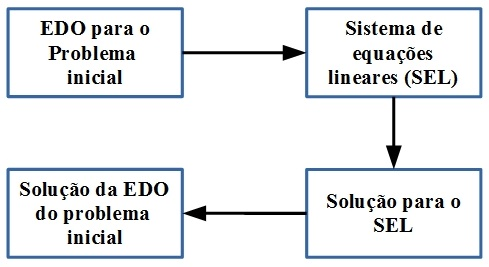
\includegraphics[scale=0.5]{EDO.jpg}
  \caption{Diagrama do algoritimo que deve ser executado quando usa-se
    de transformadas integrais para solucionar algum problema. Nesse
    caso, nosso problema considerado é a de determinar a solução de uma
    EDO via transformadas de Laplace, mas o algoritmo é genérico.}
  \label{EDO}
\end{figure}

A transformada integral de nosso interesse está associado ao formalismo
das Transformadas de Laplace (TL). Aqui discutiremos sobre as TL de
forma objetiva, bem como resultados e propriedades relevantes para este
trabalho.

\begin{defi}
  Seja $f:[0,\infty) \longrightarrow \mathbb{R}$ uma função integrável
  para todo subintervalo finito de $\left[ 0,\infty\right) $. A
  transformada de Laplace da função $f$, denotada por
  $\mathcal{L}[f(t)]$ ou $F(\xi)$, é definida por
  \begin{equation}
    F(\xi)=\int\limits_{0}^{\infty}e^{-\xi t}f(t)dt=\lim_{n \to \infty}\left[\int\limits_{0}^{n}e^{-\xi t}f(t)dt\right] \text{ ,}
  \end{equation}
  que resulta em uma função do parâmetro $\xi$.
\end{defi}

A primeira propriedade da transformada de Laplace $\mathcal{L}$ é a
linearidade, logo se
$\left\lbrace f_{i}(t)\right\rbrace = \left\lbrace
  f_{1}(t),\cdots,f_{m}(t)\right\rbrace $ com $i=1,\cdots,m$ é um
conjunto de funções cujas transformadas de Laplace existem, então
\begin{equation}
  \mathcal{L}\left[\sum_{i=1}^{m}a_{i}f_{i}(t)\right]= \sum_{i=1}^{m}a_{i}\mathcal{L}\left[f_{i}(t) \right] \text{ .} \label{linear}
\end{equation}

Uma aplicação notável das transformadas de Laplace é na resolução de
equações diferenciais ordinárias com coeficientes constantes sujeitas à
condições de contorno. Isso decorre do seguinte teorema \cite{Arfken}
\begin{theorem} \label{Teo1} Seja $f\left( t\right) $ uma fun\c{c}\~{a}o
  tal que sua $n$%
  -\'{e}sima derivada com rela\c{c}\~{a}o ao par\^{a}metro $t$ seja
  integr\'{a}%
  vel e dado um conjunto de condi\c{c}\~{o}es de contorno
  $d^{n}f\left( 0\right) /dt^{n}=c_{n}$ para todo $n$. Ent\~{a}o%
  \begin{equation}
    \mathcal{L}\left[ \frac{d^{n}f\left( t\right) }{dt^{n}}\right] \equiv \xi^{n}%
    \mathcal{L}\left[ f\left( t\right) \right] -\sum_{j=1}^{n}\xi^{n-j}c_{j-1} \text{ ,}  \label{TransfDerN}
  \end{equation}%
  onde $\mathcal{L}\left[ f\left( t\right) \right] $ \'{e} a
  transformada de Laplace de $f\left( t\right)$.
\end{theorem}

O resultado acima em conjunto com a propriedade de linearidade das
transformadas de Laplace podem ser usados para encontrar
solu\c{c}\~{o}es de sistemas de ED de ordem $n$. De fato, considere um
sistema de equa\c{c}\~{o}es diferenciais nas fun\c{c}\~{o}es
$x_{i}\left( t\right) $ e com condi\c{c}%
\~{o}es de contorno $d^{n}x_{i}\left( 0\right) /dt^{n}=c_{n}^{i}$. A
partir da Eq. (\ref{TransfDerN}) podemos concluir que aplicando a
transformada a um sistema de ED, reca\'{\i}mos em um problema de
encontrar solu\c{c}\~{o}es de sistemas de equa\c{c}\~{o}es lineares nas
vari\'{a}veis $%
\chi _{i}\left( \xi\right) =\mathcal{L}\left[ x_{i}\left( t\right)
\right] $.  Ent\~{a}o, desde que o sistema de equa\c{c}\~{o}es lineares
associados ao sistema de ED nos forne\c{c}a solu\c{c}\~{o}es
integr\'{a}veis $\chi _{i}\left( \xi\right) $, podemos usar a
transformada de Laplace inversa e obter as solu\c{c}\~{o}es
$x_{i}\left( t\right) $ do sistema de ED.

\section{Tratamento Clássico} \label{Classico} Nesta seção descreveremos
o tratamento clássico da dinâmica de uma partícula sujeita a campos
elétrico $\vec{E}$ e magnético $\vec{B}$ estáticos. Para isso,
definiremos o problema a ser tratado classicamente e em seguida
determinaremos a equação de movimento do sistema. Além disso nós
determinamos, de forma unívoca com ajuda de condições iniciais, a
solução paramétrica para a equação de movimento, onde nosso parâmetro é
o tempo $t$ de evolução do sistema. Em seguida estudaremos o
comportamento do sistema em casos particulares fazendo considerações
relacionadas aos campos $\vec{E}$ e $\vec{B}$ e as condições iniciais do
sistema.

\subsection{Solução das Equações de Movimento: Caso
  Geral} \label{Solucao}

Considere uma part\'{\i}cula de massa $m$ e carga el\'{e}trica
l\'{\i}quida $%
q$ que est\'{a} imersa em uma regi\~{a}o que, no instante $t=t_{0}$,
fica submetida à ação de dois campos est\'{a}ticos, um de natureza
magn\'{e}tica $%
\vec{B}$ e outro de natureza el\'{e}trica $\vec{E}$. J\'{a} \'{e} sabido
que cada um destes campos, a depender das condi\c{c}\~{o}es sobre a
posi\c{c}%
\~{a}o e a velocidade da part\'{\i}cula em $t=t_{0}$, exercer\'{a} uma
for%
\c{c}a sobre a part\'{\i}cula, de modo que em geral a for\c{c}a
resultante \'{e} dada pela for\c{c}a de Lorentz%
\begin{equation}
  \vec{F}_{Lor}=q\vec{E}+q\vec{v}\times \vec{B} \text{ .} \label{resultante}
\end{equation}

Sem perda de generalidade n\'{o}s adotamos que o nosso sistema de
coordenadas tem o eixo $Z$ orientado na dire\c{c}\~{a}o do campo
$\vec{B}$ e que a configura\c{c}\~{a}o incial do sistema, quando
acionamos os campos est\'{a}%
ticos, tem a forma representada pela Fig. \ref{Esquemainicial}.

\begin{figure}[!htb]
  \centering 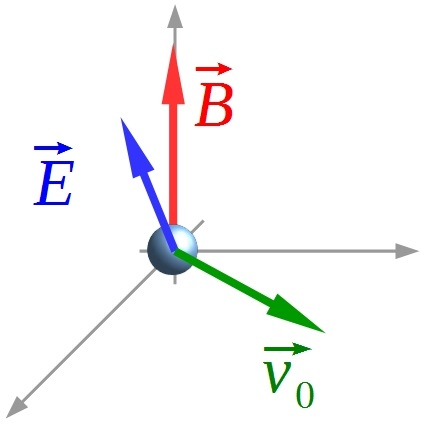
\includegraphics[scale=0.3]{Esquemainicial.jpg}
  \caption{Configuração inicial do sistema, onde estamos adotando nosso
    sistemas de coordenadas no ponto onde a partícula se encontra
    inicialmente.}
  \label{Esquemainicial}
\end{figure}


A origem do nosso sistema de coordenadas est\'{a} fixada exatamente no
ponto onde a part\'{\i}cula se localiza em $t=0 $, de modo que as
condi\c{c}\~{o}es iniciais são
\begin{equation}
  \vec{r}\left(
    0\right) =\left( 0,0,0\right) \text { \ e \ } \vec{v}\left( 0\right) =\left(v_{1}(0) ,v_{2}(0) ,v_{3}(0) \right) \text{ ,} \label{initialconditions}
\end{equation}
que é o m\'{a}ximo de simplifica\c{c}\~{a}o que conseguimos admitir sem
perder a generalidade do problema. Assim, as componentes da
acelera\c{c}\~{a}o do sistema na forma diferencial s\~{a}o dadas, de
acordo com a 2ª lei de Newton, por%
\begin{eqnarray}
  \frac{d^{2}x_{1}\left( t\right) }{dt^{2}} &=&\frac{q}{m} \left( \frac{dx_{2}\left(
                                                t\right) }{dt}B+E_{1} \right) \label{dx1} \text{ ,} \\
  \frac{d^{2}x_{2}\left( t\right) }{dt^{2}} &=&-\frac{q}{m} \left( \frac{dx_{1}\left(
                                                t\right) }{dt}B-E_{2} \right) \label{dx2} \text{ ,} \\
  \frac{d^{2}x_{3}\left( t\right) }{dt^{2}} &=&\frac{qE_{3}}{m}  \label{dx3}
\end{eqnarray}%
onde rotulamos as componentes $x,y$ e $z$ por $1,2$ e $3$,
respectivamente.  As Eqs. (\ref{dx1}) e (\ref{dx2}) claramente formam um
sistema de equa\c{c}\~{o}es diferenciais acopladas, mas por outro lado
vemos que a Eq. (\ref{dx3}) est\'{a} desacoplada das demais. Assim
n\'{o}s iniciamos por determinar a solu\c{c}\~{a}o da Eq. (\ref{dx3})
onde, por integração, facilmente podemos mostrar que%
\begin{equation}
  x_{3}\left( t\right) = v_{3} t+\frac{qE_{3}}{m}%
  \frac{t^{2}}{2} \text{ ,} \label{x3}
\end{equation}%
onde denotaremos de agora em diante a notação $\beta_{k}(0)=\beta_{k}$,
\'{e} solu\c{c}\~{a}o da Eq. (\ref{dx3}), dando assim o comportamento da
part\'{\i}cula ao longo do eixo $Z$ do sistema de
coordenadas. Continuando, para sistema composto pelas Eqs. (\ref{dx1}) e
(\ref{dx2}) n\'{o}s usamos o método da transformada de Laplace descrito
na seção \ref{Laplace}. Aplicando a transformada de Laplace às
Eqs. (\ref{dx1}) e (\ref{dx2}) obtemos, de acordo com o Teorema
\ref{Teo1} e as Eqs. (\ref{linear}) e (\ref{initialconditions})
\begin{eqnarray}
  \xi^{2}\chi _{1}\left( \xi\right) -v_{1}  &=&\frac{q}{m}%
                                                \left( B\xi\chi _{2}\left( \xi\right) +\frac{E_{1}}{\xi} \right) \text{ ,} \\
  \xi^{2}\chi _{2}\left( \xi\right) -v_{2}  &=&-\frac{q}{m}%
                                                \left( B\xi\chi _{1}\left( \xi\right) - \frac{qE_{2}}{\xi} \right) \text{ ,}
\end{eqnarray}%
onde a partir daqui vamos definir $\omega _{0}=qB/m$ e
$\gamma _{k}=qE_{k}/m$ com $k=1,2$. Para resolver o sistema acima
n\'{o}s primeiro resolvemos o sistema para $\chi _{1}\left( \xi\right) $
e $\chi _{2}\left( \xi\right) $ e em seguida aplicamos a transformada de
Laplace inversa $(5)$ para obtermos as soluções $%
x_{1}\left( t\right) $ e $x_{2}\left( t\right) $, respectivamente. O
resultado dessa sequencia de passos \'{e} que a solu\c{c}\~{a}o para as
Eqs. (\ref%
{dx1}) e (\ref{dx2}) s\~{a}o, respectivamente, dadas por%
\begin{eqnarray}
  x_{1}\left( t\right)  &=&\frac{1}{\omega_{0} ^{2}}\left[ A_{1}-C_{2}\cos \left(
                            \omega_{0} t\right) +C_{1}\sin \left( \omega_{0} t\right) \right] \text{ ,}  \label{x1} \\
  x_{2}\left( t\right)  &=&\frac{1}{\omega_{0} ^{2}}\left[ A_{2}+C_{1}\cos \left(
                            \omega_{0} t\right) +C_{2}\sin \left( \omega_{0} t\right) \right]  \text{ ,} \label{x2}
\end{eqnarray}%
onde definimos as quantidades (com $k=\{ 1,2 \}$)
\begin{eqnarray}
  A_{1} &=&\gamma _{2}+\left( \gamma _{1}t+v_{2} \right) \omega_{0} \text{ ,}
            \label{coe1} \\
  A_{2} &=&\gamma _{1}-\left( \gamma _{2}t+v_{1} \right) \omega_{0} \text{ ,}
            \label{coe2} \\
  C_{k} &=&\left( -1\right) ^{k}\gamma _{k}+v_{k} \omega_{0} \text{ ,}
            \label{coe3}
\end{eqnarray}%
de forma que uma an\'{a}lise dimensional mostra que
$\left[ A_{k}/\omega_{0} ^{2}\right] =\left[ C_{k}/\omega_{0}
  ^{2}\right] =\left[ \text{posi\c{c}\~{a}o}\right] $.  Isso nos permite
concluir que a part\'{\i}cula descreve uma trajet\'{o}ria dada pelas
equações param\'{e}tricas (\ref{x1}), (\ref{x2}) e (\ref{x3}). Das
Eqs. (\ref{coe1}), (\ref{coe2}) e (\ref{coe3}) podemos ver que, de fato,
a configura\c{c}\~{a}o dos campos e a condi\c{c}\~{a}o inicial
$\vec{v}\left( 0\right) $ afetam diretamente a trajet\'{o}ria da
part\'{\i}cula, dando-nos uma gama de possibilidades para sua
trajet\'{o}ria.

\subsection{Casos Particulares} \label{Particular}

Levando em conta que a configuração dos campos e a condição inicial
$\vec{v}\left( 0\right) $ tem influência direta na trajetória da
partícula, vamos considerar casos particulares de trajetórias que podem
ser obtidas mediante certas condições inicias aplicadas às equações
paramétricas (\ref{x1}), (\ref{x2}) e (\ref{x3}) que descrevem a
trajetória geral da partícula.

\begin{itemize}
\item \textbf{Caso particular 1}
\end{itemize}
% \subsection*{1º Caso:}

Inicialmente, vamos considerar o caso em que a partícula entra numa
região contendo apenas o vetor campo magnético de tal forma que
$\vec{v}(0)\perp\vec{B}$ com
$\vec{v}(0) = \vec{v}_{0} =(v_{1},v_{2},0)$. Neste caso, as equações
paramétricas (\ref{x1}) e (\ref{x2}) tomam a seguinte forma
\begin{eqnarray}
  x_{1}\left( t\right)  &=&\frac{1}{\omega_{0}}\left[v_{2} (1 - \cos \left(\omega_{0} t\right)) + v_{1}\sin \left( \omega_{0} t\right) \right] \label{circularx} , \\
  x_{2}\left( t\right)  &=&\frac{1}{\omega_{0}}\left[ v_{1}(1 + \cos \left(
                            \omega_{0} t\right)) + v_{2}\sin \left( \omega_{0} t\right) \right] , \label{circulary}
\end{eqnarray}%
que podem ser postas facilmente na forma
\begin{equation}
  \left( x_{1}(t) - \dfrac{v_{2}}{\omega_{0}}\right) ^{2} + \left( x_{2}(t) - \dfrac{v_{1}}{\omega_{0}}\right) ^{2} = \dfrac{\Arrowvert \vec{v}_{0}\Arrowvert^{2}}{\omega_{0}^{2}} \text{ ,} \label{c1}
\end{equation}
que é a equação de uma circunferência de raio
$R=\vert \vert \vec{v}\vert \vert / \omega_{0}$ centrada no ponto
$\left( v_{2} / \omega_{0},v_{1} / \omega_{0}\right) $ e onde
$\vert \vert \vec{v} \vert \vert = (v_{1}^2 + v_{2}^2)^{\frac{1}{2}}$ é
a norma da velocidade inicial da carga. Em outras palavras, a
Eq. (\ref{c1}) mostra que a partícula executa um movimento circular no
plano $xy$ com raio $R=\vert \vert \vec{v}\vert \vert /\omega_{0}$.

A fim de dar uma descrição mais completa do movimento, considere o vetor
posição da partícula $\vec{r}(t)$ no instante $t$ como
$\vec{r}(t)=x_{1}(t) \hat{\text{i}} + x_{2}(t) \hat{\text{j}} $, com
$\hat{i}$ e $\hat{j}$ sendo versores na direção $x$ e $y$,
respectivamente. Então, o vetor velocidade $\vec{v}(t)$ da partícula é
dado por
\begin{equation}
  \vec{v}(t) = \frac{d \vec{r}(t)}{dt} = \dot{x}_{1}(t) \hat{\text{i}} + \dot{x}_{2}(t) \hat{\text{j}} = v_{1}(t) \hat{\text{i}} + v_{2}(t) \hat{\text{j}} \text{ ,}
\end{equation}
onde
\begin{eqnarray}
  v_{1}(t) &=& v_{2} \sin (\omega _{0} t) + v_{1} \cos (\omega _{0} t) \text{ ,} \\
  v_{2}(t) &=& v_{2} \cos (\omega _{0} t) - v_{1} \sin (\omega _{0} t) \text{ ,}
\end{eqnarray}
com a norma do vetor $\vec{v}(t)$ sendo
$\vert \vert \vec{v}(t) \vert \vert = \vert \vert \vec{v_{0}}\vert
\vert$, para todo instante do movimento, configurando assim um movimento
circular com velocidade de módulo constante. Portanto, podemos agora
assumir $\omega_{0}$ como sendo a frequência angular do movimento
circular que é executado pela partícula.

\begin{itemize}
\item \textbf{Caso particular 2}
\end{itemize}
% \subsection*{2º Caso:}

Vamos considerar agora a configuração tal que a carga é lançada
obliquamente às linhas de indução de $\vec{B}$, considerando
$\vec{E}=\vec{0}$ e $\vec{v}_{0} = (v_{1},0,v_{3})$. Nesse caso, usando
as Eqs. (\ref{x3}), (\ref{x1}), (\ref{x2}) e explicitando $A_{1}$,
$A_{2}$, $C_{1}$ e $C_{2}$ em termos das configurações dadas para
$\vec{B}$, $\vec{E}$ e $\vec{v}_{0}$ temos:
\begin{eqnarray}
  x_{1}\left( t\right)  &=& \rho_{L} \sin \left(
                            \omega_{0} t\right)  \label{HL1} \text{ ,} \\
  x_{2}\left( t\right)  &=& \rho_{L} \left[ 1 + \cos \left(
                            \omega_{0} t\right) \right]   \label{HL2}\\
  x_{3}\left( t\right) &=& v_{3} t \text{ ,} \label{HL3}
\end{eqnarray}%
onde $\rho_{L} = m v_{1} / \vert q \vert B$ é conhecido na literatura
como raio de Larmor. As Eqs. (\ref{HL1}), (\ref{HL2}) e (\ref{HL3})
mostram que, nestas condições, a partícula descreve uma trajetória
helicoidal equivalente à composição de um movimento circular com
velocidade constante %$v_{0\perp}=
$v_{1}$ e raio $\rho_{L}$ no plano
$xy$ e de um movimento com velocidade constante %$v_{0\parallel}=
$v_{3}$ na direção das linhas de indução. A este movimento dar-se o nome
de giração e o centro do movimento circular que, nesse caso, possui
coordenadas $(x,y,z)=(0,\rho_{L},0)$, denomina-se centro de guia. Nesse
caso, o centro de guia desloca-se com velocidade constante $v_{3}$ na
direção das linhas de indução de forma que a giração é um circulo cuja
equação no plano $xy$ é dada pela Eq. (\ref{c1}) tomando $v_{2}=0$
\cite{Viana}.

\begin{figure}[!htb]
  \centering 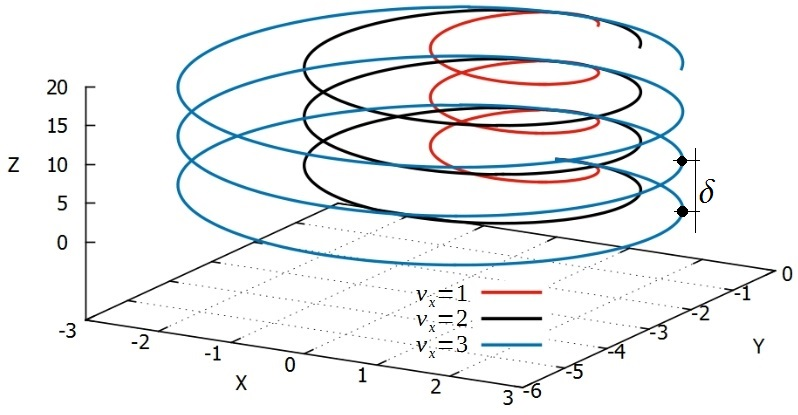
\includegraphics[scale=0.38]{Helicoidal.jpg}
  \caption{Trajetória helicoidal da partícula resultante da
    particularização no caso 2. A escolha dos parâmetros que configuram
    os campos para construir o gráfico foram
    $(\gamma_1,\gamma_2,\gamma_3,\omega_0)=(0,0,0,1)$ (estamos adotando
    unidades de medidas no SI). As curvas estão associadas a diferentes
    escolhas para a componente $x$ da velocidade inicial e fixamos a
    componente $z$ como a unidade.}
  \label{helicoidal}
\end{figure}

Considerando a velocidade $\vec{v}$ da partícula ao longo da trajetória
helicoidal e definindo o ângulo de passo $\phi$ de tal forma que as
componentes de $\vec{v}$ nas direções paralela e perpendicular a
$\vec{B}$ sejam dadas por
\begin{eqnarray}
  v_{3} &=& \|\vec{v}\| \cos \left(\phi\right) \text{ ,} \label{AP1} \\
  v_{2} &=& \|\vec{v}\| \sin \left(\phi\right)  \text{ ,} \label{AP2}
\end{eqnarray}%
então o passo da hélice $\delta$ será definido como a distância
percorrida pela partícula na direção paralela a $\vec{B}$ a cada período
do movimento circular $\tau = \frac{2\pi}{\omega_{0}}$, ou seja
\begin{eqnarray}
  \delta &=& \tau v_{3} = \frac{2 \pi \|\vec{v}\|}{\omega_{0}}  \cos \left(\phi\right) \text{ .} \label{PS1}
\end{eqnarray}%

Na Fig. \ref{helicoidal} podemos visualizar a trajetória da partícula,
onde a distância vertical entre dois pontos da trajetória (como
sinalizado na curva em azul) é dado pela quantidade $\delta$ discutida
acima.

\begin{figure}[!htb]
  \centering 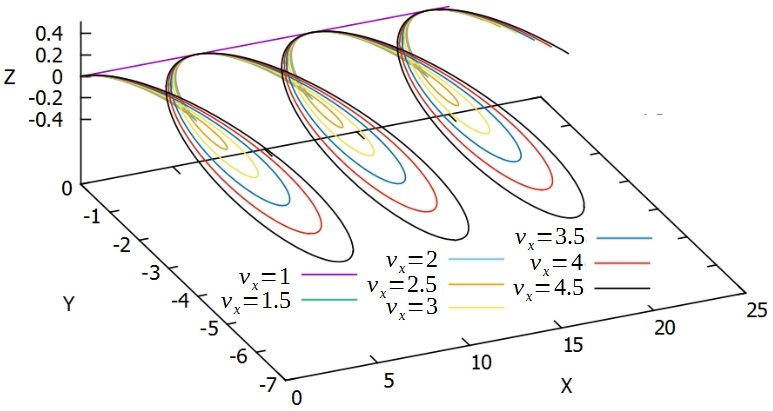
\includegraphics[scale=0.4]{Graph1.jpg}
  \caption{Trajetória da partícula como resultado da particularização no
    caso 3. Novamente a escolha dos parâmetros para construir o gráfico
    se dá como $(\gamma_1,\gamma_2,\gamma_3,\omega_0)=(1,0,0,1)$. A
    única componente da velocidade é na direção $x$ e plotamos o gráfico
    para várias escolhas deste a fim de visualizar os pontos fixos
    independentes da velocidade inicial. Unidades de medidas novamente
    no SI.}
  \label{Graph1}
\end{figure}

\begin{itemize}
\item \textbf{Caso particular 3}
\end{itemize}
% \subsection*{3º Caso:}

Agora vamos considerar o caso em que a partícula entra numa região na
qual estão presentes os campos elétrico e magnético cruzados tais que
$\vec{E}=(E_{1},0,0)$, $\vec{B}=(0,0,B)$ e
$\vec{v}_{0}=(v_{1},0,0)$. Com estas configurações podemos simplificar
as Eqs. (\ref{x1}) e (\ref{x2}) que tomam a forma
\begin{eqnarray}
  x_{1}\left( t\right)  &=&\frac{1}{\omega_{0} ^{2}}\left[ A_{1} +C_{1}\sin \left( \omega_{0} t\right) \right] \label{cx} \text{ ,}  \\
  x_{2}\left( t\right)  &=&\frac{1}{\omega_{0} ^{2}}\left[ A_{2}+C_{1}\cos \left(
                            \omega_{0} t\right) \right]  \text{ .} \label{cy}
\end{eqnarray}%

Explicitando $A_{1}$, $A_{2}$ e $C_{1}$ em termos das configurações
dadas para $\vec{E}$, $\vec{B}$ e $\vec{v}_{0}$ obtemos
\begin{eqnarray}
  x_{1}\left( t\right)  &=& \frac{qE_{1}}{m \omega_{0}}\left[t +\left( \frac{mv_{1}}{qE_{1}}-\frac{1}{\omega_{0}} \right)\sin \left( \omega_{0} t\right) \right] \label{cx1} , \\
  x_{2}\left(t\right)&=&\frac{1}{\omega_{0}^{2}}\left[(\frac{qE_{1}}{m}-\omega_{0}v_{1})(1 - \cos\left(\omega_{0}t\right))\right] , \label{cy1}
\end{eqnarray}%
de forma que se $v_{1}=0$ obtemos
\begin{eqnarray}
  x_{1}\left( t\right)  &=&\frac{qE_{1}}{m\omega_{0} ^{2}}\left[\omega_{0} t - \sin \left( \omega_{0} t\right) \right] \label{cx2}  \text{ ,}  \\
  x_{2}\left(t\right)&=&\frac{qE_{1}}{m\omega_{0}^{2}}\left[ 1  -\cos\left(\omega_{0}t\right)\right] \text{ ,}
                         \label{cy2}
\end{eqnarray}%
que são exatamente as equações paramétricas de uma cicloide com $t$
atuando como parâmetro.

É interessante notar aqui a existência de um efeito de focalização
\cite{Simoes} que ocorre nesse tipo de trajetória e que obriga a
partícula eletrizada a passar por uma sucessão de pontos fixos no eixo
$X$, chamados de pontos focais, independentemente do valor da velocidade
inicial $v_{0}$. Podemos mostrar isso tomando o conjunto de valores de
$t$ que satisfaz $x_{2}=0$ na Eq. (\ref{cy1}), que implica em ter
$\cos\left(\omega_{0}t\right)=1$, de modoq que podemos construir a
família de valores $t= 2 \pi\lambda / \omega_{0}$ com
$\lambda \in \mathbb{Z}$. Substituindo esse valor de $t$ na
Eq. (\ref{cx1}), obtemos
\begin{equation}
  x_{1}= 2\pi \lambda \dfrac{ q E_{1}}{\omega_{0}^2 m} = 2\pi \lambda \dfrac{ m E_{1}}{q B^2} \text{ ,}
  \label{pf}
\end{equation}
onde na ultima igualdade usamos que $\omega_{0}= qB / m$. A equação
acima fornece a posição dos pontos focais ao longo do eixo $X$, como
pode ser visto na Fig. \ref{Graph1}.

\section{O Tratamento Quântico} \label{Quantico}

Agora n\'{o}s mostraremos como tratar um sistema qu\^{a}ntico cujo seu
an%
\'{a}logo cl\'{a}ssico foi discutido anteriormente na se\c{c}\~{a}o
\ref{Classico}. O que faremos aqui nada mais \'{e} do que uma
aproxima\c{c}\~{a}o na tentativa de descrever a din\^{a}mica de um feixe
de part\'{\i}culas cuja din\^{a}mica de cada part\'{\i}cula que contitui
o sistema \'{e} dada pela equa\c{c}\~{a}o de Schr%
\"{o}dinger. Para tal, iremos utilizar o conhecido \textit{%
  Teorema de Ehrenfest} \cite{Ehrenfest}. Com rela\c{c}\~{a}o aos
resultados relacionados ao Teorema de Ehrenfest, aqui n\'{o}s faremos
algo bastante resumido e focado no nosso objetivo, para uma
discuss\~{a}o mais geral recomendamos a \cite{Bolivar}, onde outras
refer\^{e}ncias sobre o assunto podem ser encontradas.

Nosso ponto de partida \'{e} a equa\c{c}\~{a}o de Schr\"{o}dinger dada
por%
\begin{equation}
  H\left( \vec{r},t\right) \left\vert \psi \left( \vec{r},t\right)
  \right\rangle =i\hbar \partial _{t}\left\vert \psi \left( \vec{r},t\right)
  \right\rangle  \text{ ,} \label{schro}
\end{equation}%
sendo $\partial _{t}$ o operador derivada parcial e onde $%
H\left( \vec{r},t\right) $ \'{e} o Hamiltoniano que governa o sistema
dado por%
\begin{equation}
  H\left( \vec{r},t\right) =\frac{\vec{p}^{2}}{2m}+V\left( \vec{r},t\right) \text{ ,}
  \label{Hamil}
\end{equation}%
com $\vec{p}=\left( \hat{p}_{x},\hat{p}_{y},\hat{p}_{z}\right) $ e
$\vec{r}%
=\left( \hat{r}_{x},\hat{r}_{y},\hat{r}_{z}\right) $ o operador momento
e posi\c{c}\~{a}o, respectivamente, em tr\^{e}s dimens\~{o}es e que
satisfazem as rela\c{c}\~{o}es de comuta\c{c}\~{a}o%
\begin{equation}
  \left[ \hat{r}_{k},\hat{p}_{m}\right] =i\hbar \delta _{km}\1\text{ \ , \ }\left[
    \hat{r}_{k},\hat{r}_{m}\right] =\left[ \hat{p}_{k},\hat{p}_{m}\right] =0 \text{ .}
  \label{comu}
\end{equation}

A equa\c{c}\~{a}o de Schr\"{o}dinger descreve a din\^{a}mica de sistemas
qu\^{a}nticos, mas existe uma maneira an\'{a}loga de analisarmos a
evolu\c{c}\~{a}o de um sistema que \'{e} analisando como evoluem os
valores esperados de algum observ\'{a}vel f\'{\i}sico. Sendo
$\mathcal{O}$ um observ%
\'{a}vel fisico (Energia, posi\c{c}\~{a}o, momento, etc...), ent\~{a}o o
valor esperado deste observ\'{a}vel \'{e} definido como%
\begin{equation}
  \left\langle \mathcal{O}\right\rangle =\left\langle \psi \left( \vec{r}%
      ,t\right) |\mathcal{O}|\psi \left( \vec{r},t\right) \right\rangle \text{ .}
\end{equation}

Derivando esta equa\c{c}\~{a}o com rela\c{c}\~{a}o ao tempo, podemos
mostrar que%
\begin{equation}
  \frac{d}{dt}\left\langle \mathcal{O}\right\rangle =\frac{i}{\hbar }%
  \left\langle \left[ H\left( \vec{r},t\right) ,\mathcal{O}\right]
  \right\rangle +\left\langle \partial _{t}\mathcal{O}\right\rangle \text{ ,}
  \label{evO}
\end{equation}%
onde estamos considerando que o operador $\mathcal{O}$ n\~{a}o possui
dependencia temporal, assim $\left\langle \partial _{t}\mathcal{O}%
\right\rangle =0$. Como a equa\c{c}\~{a}o acima envolve m\'{e}dias de
uma quantidade f\'{\i}sica, ent\~{a}o devemos atentar para o fato de que
estamos tratando de um grande n\'{u}mero de medidas do observ\'{a}vel
$\mathcal{O}$, ou para um ensemble de part\'{\i}culas (feixe de
el\'{e}trons, f\'{o}tons, etc).

Agora deixe-nos analisar os resultados que podemos obter da
Eq. (\ref{evO}) no caso particular de nosso interesse, ou seja, uma
part\'{\i}cula de carga $q$ sujeito à ação de um campo
eletromagn\'{e}tico. Já é sabido que o Hamiltoniano que governa a
dinâmica desse sistema é dado por \cite{Sakuray:book}
\begin{equation}
  H\left( \vec{r}\right) =2m\left[ \vec{p}-q\vec{A}\left( \vec{r},t\right) %
  \right] ^{2}+q\phi \left( \vec{r},t\right) \text{ ,}  \label{HSis}
\end{equation}%
onde $\vec{A}\left( \vec{r},t\right) $ e $\phi \left( \vec{r},t\right) $
s%
\~{a}o os potenciais vetor e escalar, respectivamente, usados para
escrever os campos el\'{e}tricos e magn\'{e}ticos, respectivamente, sob
a forma%
\begin{eqnarray}
  \vec{E}\left( \vec{r},t\right)  &=&-\vec{\nabla}\phi \left( \vec{r},t\right)
                                      -\partial _{t}\vec{A}\left( \vec{r},t\right) \text{ ,}  \label{E} \\
  \vec{B}\left( \vec{r},t\right)  &=&\vec{\nabla}\times \vec{A}\left( \vec{r}%
                                      ,t\right)  \text{ .} \label{B}
\end{eqnarray}

Usando um algebrismo um pouco extenso e as rela\c{c}\~{o}es de
comuta\c{c}%
\~{a}o na Eq. (\ref{comu}), bem como as equa\c{c}\~{o}es acima, n%
\'{o}s podemos mostrar que para o Hamiltoniano da Eq. (\ref{HSis})
n\'{o}s temos
\begin{equation}
  m\frac{d^{2}}{dt^{2}}\left\langle \vec{r}\right\rangle =q\left[ \vec{E}+%
    \frac{d}{dt}\left\langle \vec{r}\right\rangle \times \vec{B}\right] \text{ ,}
  \label{ResulQuant}
\end{equation}%
de modo que devemos olhar para a quantidade $\left\langle \vec{r}%
\right\rangle $ como
$\left\langle \vec{r}\right\rangle =\left\langle \hat{x}%
\right\rangle \hat{\imath}+\left\langle \hat{y}\right\rangle
\hat{\jmath}%
+\left\langle \hat{z}\right\rangle \hat{k}$, onde $\left\langle \hat{m}%
\right\rangle $ \'{e} o valor esperado do operador associado \`{a}
$\hat{m}$-%
\'{e}sima coordenada da "posi\c{c}\~{a}o" da part\'{\i}cula.

A Eq. (\ref{ResulQuant}) mostra que o comportamento do valor esperado de
$\vec{r}$ é descrito por equações de movimento semelhante a
Eq. (\ref{resultante}) (como esperado do Teorema de Ehrenfest)
considerando, é claro, que os campos $\vec{E}$ e $\vec{B}$ s\~{a}o
uniformes (independentes da posi\c{c}\~{a}o). Esse resultado nos d\'{a}
a equa\c{c}\~{a}o de movimento para um ensemble de part\'{\i}culas, cuja
carga do ensemble \'{e} $q$, na presen\c{c}a de campos magn\'{e}tico e
el\'{e}trico est\'{a}ticos e uniformes, e será de maior import\^{a}ncia
para estudos mais avançados que serão desenvolvidos posteriormente.

% \begin{figure}[!t]
%   \centering \includegraphics[scale=0.3]{Regime2.png}
%   \caption{Gráfico da quantidade $Q^{-1}\left( a,m \right)$
%   considerando que $\omega _{0}\gg \omega
%   _{T}$. %A curva foi construída considerando que $\alpha=10$}
%   \label{graph2}
% \end{figure}

\section{Conclusão}

A partir da transformada de Laplace estudamos o caso mais geral da
dinâmica de uma partícula sujeita a interação com campos elétrico e
magnético estáticos. Usando a definição e propriedades da transformada
de Laplace, mostramos como mapear o problema de resolver um sistema de
equações diferenciais ordinárias em um problema de encontrar a solução
de um sistema de equações lineares de primeiro grau. Com isso,
encontramos a solução mais geral possível da equação de movimento que
rege a dinâmica do sistema em termos das componentes dos vetores
$\vec{B}$, $\vec{E}$ e $\vec{v}(0)$ onde, a partir da solução geral,
mostramos como obter a solução de três casos particulares cuja
importância e aplicabilidade excedem o ponto de vista didático. Por fim,
motivamos o nosso estudo fazendo o tratamento quântico do sistema
estudado, onde consideramos um feixe de partículas sem spin
carregadas. Nesse contexto, mostramos que a curva parametrizada do valor
esperado (em média) do vetor posição de uma partícula do feixe em função
do tempo corresponde aquela curva associada ao seu análogo clássico.

A consideração de campos $\vec{B}$ e $\vec{E}$ estáticos nos permite
mostrar que a dinâmica do sistema é dada por um sistema de equações
diferenciais acopladas com coeficientes constantes. No entanto, algumas
outras situações não foram discutidas, como o caso de campos não
estáticos, de modo que alguns fenômenos não foram levados em
consideração, como o potencial retardado criado pela corrente elétrica
devido ao movimento da carga \cite{Jackson}. Além disso, existem uma
gama de dinâmicas cuja solução pode ser analisada por meio de
transformadas integrais e que são de interesse mais amplo, como a
solução da Eq. de Lindblad \cite{Nielsen:Book} que descreve a dinâmica
de sistemas quânticos sob influências do ambiente (decoerência). Todas
essas situações não discutidas aqui serão as motivações de nossos
desenvolvimentos futuros, uma vez que a dinâmica agora deve passar a ser
regida por um sistema de equações diferenciais acopladas com maior
número de equações e onde podemos ter coeficientes de acoplamento
dependentes do tempo e/ou posição.

\section*{Agradecimentos}

A.C.S. gostaria de agradecer ao Conselho Nacional de Desenvolvimento
Científico e Tecnológico (CNPq) e ao Instituto Nacional de Ciência e
Tecnologia de Informação Quântica (INCT-IQ) pelo suporte financeiro a
esse projeto. M.L.M. agradece ao departamento de Física da Universidade
Regional do Cariri - URCA.

\begin{thebibliography}{99}
  \bibliographystyle{unsrt}

\bibitem{Sommerfeld} A. Sommerfeld, \textit{Lectures on Theoretical
    Physics vol. 1}, (Academic Press Inc, New York, 1952), 3th ed.

\bibitem{Landau} L.D. Landau and E.M. Lifchitz, \textit{Course of
    Theoretical Physics vol. 1}, (Elsevier, New York, 1976), Third
  edition.

\bibitem{Griffiths} D. J. Griffiths, \textit{Introduction to
    Electrodynamics}, (Prentice Hall, New Jersey, 1999), 3th ed.

\bibitem{Moyses} H. M. Nusseszveig, \textit{Curso de Física Básica
    vol. 3}, (Blücher, São Paulo, 1997), 1ª ed.

\bibitem{Marion} Thornton, S. T., Marion, J. B., \textit{Classical
    Dynamics of Particles and Systems}, (Thomson Learning, Belmont,
  2004), 5th ed.

\bibitem{Moyses2} H. M. Nusseszveig, op. cit., pag. 129.

\bibitem{Natascha:16} {N. Riahi}, e-print: arXiv:1606.07713 (2016).

\bibitem{Ref1Natascha:16} B. U. Felderhof, Journal of Physics A
  \textbf{41}, 445302 (2008).

\bibitem{Ref2Natascha:16} G. G.-Calderon and A. Rubio, Phys. Rev. A
  \textbf{55}, 3370 (1997).

\bibitem{Arfken} G. B. Arfken and H. J. Weber, \textit{Física
    Matemática}, (Elsevier, Rio de Janeiro, 2007), 6ª ed. op. cit.,
  pag. 736.

\bibitem{Viana} R. L. Viana, \textit{Introdução à Eletrodinâmica
    Clássica}. Universidade Federal do Paraná, (2012),(Apostila),
  pag. 209.

\bibitem{Simoes} C. S. Pereira, \textit{Processo de Attachment,
    Densidade de Raios e a Ocorrência de Flashover em Linhas de
    Transmissão de Eletricidade}. Universidade Federal do Pará, (2014),
  pag. 98.

\bibitem{Ehrenfest} P. Ehrenfest, \textit{Bemerkung über die angenärte
    Gültigkeit der klassischen Mechanik innerhalb der Quantenmechanik},
  Zeitschrift für Physik \textbf{45}, 445 (1927).

\bibitem{Bolivar} A. O. Bolivar, \textit{Teorema de Ehrenfest e o Limite
    Clássico da Mecânica Quântica}, Rev. Bras. Ensino Fís. \textbf{23},
  190 (2001).

\bibitem{Sakuray:book} J. J. Sakuray, \textit{Modern Quantum Mechanics}
  (Addison-Wesley, US, 1995), Rev. ed.

\bibitem{Jackson} J. D. Jackson, \textit{Classical Electrodynamics},
  (John Wiley and Sons, New York, 1962), Third edition.

\bibitem{Nielsen:Book} M. A. Nielsen and I. L. Chuang, \textit{Quantum
    Computation and Quantum Information}, Cambridge University Press,
  Reino Unido, (2000).

\end{thebibliography}

\end{document}
